\documentclass{standalone}
\usepackage{tikz}
\usepackage{ctex,siunitx}
\setCJKmainfont{Noto Serif CJK SC}
\usepackage{tkz-euclide}
\usepackage{amsmath}
\usetikzlibrary{patterns, calc,3d}
\usetikzlibrary {decorations.pathmorphing,decorations.pathreplacing,decorations.shapes,}
\begin{document}
\small
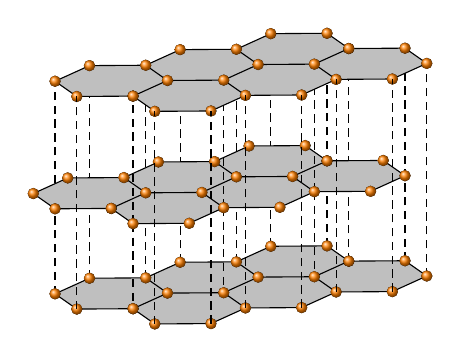
\begin{tikzpicture}[>=latex,scale=1.35,z={(190:10mm)},x={(-35:5mm)}]
  % \useasboundingbox(-1.0,-1.4)rectangle(3.5,3.7);
  \foreach \x/\z in { 1.00/-1.732, 0.50/-1.732, 0.25/-1.299,-0.25/-1.299,-0.50/-0.866,-0.25/-0.433,-0.50/ 0.000,-0.25/ 0.433,-0.50/ 0.866,-0.25/ 1.299}
  {
    \draw[densely dashed](\x,0,\z)--(\x,2,\z);
  }
  \draw[fill=lightgray]( 1.25,0,-1.299)--( 1.00,0,-1.732)--( 0.50,0,-1.732)--( 0.25,0,-1.299)--(-0.25,0,-1.299)--(-0.50,0,-0.866)--(-0.25,0,-0.433)--(-0.50,0, 0.000)--(-0.25,0, 0.433)--(-0.50,0, 0.866)--(-0.25,0, 1.299)--( 0.25,0, 1.299)--( 0.50,0, 0.866)--( 1.00,0, 0.866)--( 1.25,0, 0.433)--( 1.00,0, 0.000)--( 1.25,0,-0.433)--( 1.00,0,-0.866)--cycle;
  \draw(0.25,0,-1.299)--(0.50,0,-0.866)--(0.25,0,-0.433)--(0.50,0, 0.000)--(0.25,0, 0.433)--(0.50,0, 0.866)(0.50,0,-0.866)--(1,0,-0.866)(0.50,0,0)--(1,0,0)(-0.25,0,-0.433)--(0.25,0,-0.433)(-0.25,0,0.433)--(0.25,0,0.433);







  \draw[fill=lightgray]( 0.75,0.8,-1.299)--( 0.50,0.8,-1.732)--( 0.00,0.8,-1.732)--(-0.25,0.8,-1.299)--(-0.75,0.8,-1.299)--(-1.00,0.8,-0.866)--(-0.75,0.8,-0.433)--(-1.00,0.8, 0.000)--(-0.75,0.8, 0.433)--(-1.00,0.8, 0.866)--(-0.75,0.8, 1.299)--(-0.25,0.8, 1.299)--( 0.00,0.8, 0.866)--( 0.50,0.8, 0.866)--( 0.75,0.8, 0.433)--( 0.50,0.8, 0.000)--( 0.75,0.8,-0.433)--( 0.50,0.8,-0.866)--cycle;
  \draw(-0.25,0.8,-1.299)--( 0.00,0.8,-0.866)--(-0.25,0.8,-0.433)--( 0.00,0.8, 0.000)--(-0.25,0.8, 0.433)--( 0.00,0.8, 0.866)( 0.00,0.8, -0.866)--( 0.50,0.8, -0.866)(0,0.8,0)--(0.5,0.8,0)(-0.25,0.8,-0.433)--(-0.75,0.8,-0.433)(-0.25,0.8,0.433)--(-0.75,0.8,0.433);

  \foreach \x/\z in {0.50/-0.866, 0.50/ 0.000, 0.50/ 0.866}
  {
    \draw[densely dashed](\x,0.8,\z)--(\x,2,\z);
  }

  \draw[fill=lightgray]( 1.25,2,-1.299)--( 1.00,2,-1.732)--( 0.50,2,-1.732)--( 0.25,2,-1.299)--(-0.25,2,-1.299)--(-0.50,2,-0.866)--(-0.25,2,-0.433)--(-0.50,2, 0.000)--(-0.25,2, 0.433)--(-0.50,2, 0.866)--(-0.25,2, 1.299)--( 0.25,2, 1.299)--( 0.50,2, 0.866)--( 1.00,2, 0.866)--( 1.25,2, 0.433)--( 1.00,2, 0.000)--( 1.25,2,-0.433)--( 1.00,2,-0.866)--cycle;
  \draw(0.25,2,-1.299)--(0.50,2,-0.866)--(0.25,2,-0.433)--(0.50,2, 0.000)--(0.25,2, 0.433)--(0.50,2, 0.866)(0.50,2,-0.866)--(1,2,-0.866)(0.50,2,0)--(1,2,0)(-0.25,2,-0.433)--(0.25,2,-0.433)(-0.25,2,0.433)--(0.25,2,0.433);

  \foreach \x/\z in {0.50/-0.866, 0.50/ 0.000, 0.50/ 0.866}
  {
    \draw[densely dashed](\x,0.8,\z)--(\x,0,\z);
  }

  \foreach \x/\z in { 1.25/-1.299, 1.00/-1.732, 0.50/-1.732, 0.25/-1.299,-0.25/-1.299,-0.50/-0.866,-0.25/-0.433,-0.50/ 0.000,-0.25/ 0.433,-0.50/ 0.866,-0.25/ 1.299, 0.25/ 1.299, 0.50/ 0.866, 1.00/ 0.866, 1.25/ 0.433, 1.00/ 0.000, 1.25/-0.433, 1.00/-0.866, 0.25/-1.299, 0.50/-0.866, 0.25/-0.433, 0.50/ 0.000, 0.25/ 0.433, 0.50/ 0.866}
  {
    \fill[ball color=orange](\x,0,\z)circle(1.5pt);
    \fill[ball color=orange](\x,2,\z)circle(1.5pt);
  }
  \foreach \x/\z in{ 0.75/-1.299, 0.50/-1.732, 0.00/-1.732,-0.25/-1.299,-0.75/-1.299,-1.00/-0.866,-0.75/-0.433,-1.00/ 0.000,-0.75/ 0.433,-1.00/ 0.866,-0.75/ 1.299,-0.25/ 1.299, 0.00/ 0.866, 0.50/ 0.866, 0.75/ 0.433, 0.50/ 0.000, 0.75/-0.433, 0.50/-0.866,-0.25/-1.299, 0.00/-0.866,-0.25/-0.433, 0.00/ 0.000,-0.25/ 0.433, 0.00/ 0.866}
  {\fill[ball color=orange](\x,0.8,\z)circle(1.5pt);}

  \foreach \x/\z in { 1.25/-1.299,0.25/ 1.299, 1.00/ 0.866, 1.25/ 0.433, 1.00/ 0.000, 1.25/-0.433, 1.00/-0.866}
  {
    \draw[densely dashed](\x,0,\z)--(\x,2,\z);
  }

\end{tikzpicture}
\end{document}